\documentclass[12pt, a4paper]{article}
\renewcommand*\contentsname{Inhaltsverzeichnis}
\usepackage[ngerman]{babel}
\usepackage{mathptmx}
\usepackage{blindtext}
\usepackage{emptypage}
\usepackage{wrapfig}
\usepackage[pdftex]{graphicx}
\usepackage{geometry}
\usepackage{multirow}
\usepackage{mathcomp}
\usepackage[version=4,arrows=pgf-filled,
textfontname=sffamily,
mathfontname=mathsf]{mhchem}
\usepackage{array}
\usepackage[table]{xcolor}
\usepackage{xcolor}
\usepackage{setspace}
\usepackage{hyperref}
\usepackage{csquotes}
\usepackage[backend=biber,style=chem-acs,sorting=none]{biblatex}
\addbibresource{literatur.bib}  % Deine .bib-Datei einbinden

\DeclareCiteCommand{\cite}
  {\usebibmacro{prenote}}
  {\textsuperscript{\printfield{labelnumber}}}
  {\multicitedelim}
  {\usebibmacro{postnote}}


 \geometry{
 a4paper,
 total={170mm,257mm},
 left=25mm,
 top=25mm,
 }
\setstretch{1.213}


\newcommand{\datum}{\day.\month.\year}
\DeclareGraphicsExtensions{.pdf,.jpeg,.png,.jpg} 

\begin{document}


\begin{figure}
    \includegraphics[scale=0.14]{Universität_Bayreuth.svg.png}
\end{figure}


%Deckblatt

{\raggedright Universität Bayreuth\\  95447 Bayreuth}


\vspace{5cm}

\begin{center}
{\LARGE\bf{Anorganische Chemie III}} \\  
\vspace{1cm}
{\Large\bf{Zeolithe}}\\
\vspace{0.5cm}
{\large Justus Friedrich\\}
{Studiengang: B.Sc. Chemie\\}
{4. Fachsemester}
\end{center}





\thispagestyle{empty}
\begin{center}
{\small Matrikelnummer: 1956010 \\
E–Mail:  bt725206@myubt.de}
\end{center}

\vspace{5cm}

\begin{center}
  \today
\end{center}


\newpage
%Inhaltsverzeichnis
\tableofcontents
\thispagestyle{empty}


%Teil 1
\newpage
\setcounter{page}{1}
\section{Einleitung}



\subsection{Einführung}
{
Zeolithe werden in der heutigen Zeit immer interessanter, da diese sehr vielseitig einsetzbar sind. 
Dies liegt an der Struktur der Zeolithe, diese ist nämlich porös. Dabei sind die Größe der Poren kleiner als 
2 nm, somit sind Zeolithe Teil der mikroporösen Materialien. Dabei ermöglichen die Poren, in der kristallinen
Struktur, dass eine selektive Katalyse stattfinden kann. Bzw. können sie als Ionenaustauscher
funktionieren, oder als Adsorptionsmittel. Dabei lässt sich die Struktur des Zeoliths durch Anpassung der Kationen 
in der Zwischenschicht verändern.\cite{riedel}
}

\subsection{Ziel des Versuchs}
{
In diesen Versuch soll das Zeolith A $\{[{Na^+}]_{96}\cdotp[216 \: H_2O]\}\{[AlO_2]_{96}[SiO_2]_{96}\}$ hergestellt werden, daraufhin soll die Kristallstruktur untersucht und 
die Ionenaustauschkapazität gemessen werden, diese sollen mit den Theoriewerten verglichen werden.\cite{Skript}
}

\newpage
%Teil2
\section{Durchführung}
\subsection{Synthese von Zeolith A}
{
Es werden zwei 0.988 $\frac{mol}{L}$ NaOH-Lösungen hergestellt. Dafür werden jeweils 
5.93 g (148 mmol) NaOH in 150 mL Wasser gelöst. Zu der ersten NaOH-Lösung wird 7.72 g (37.1 mmol) {Tetraethoxysilan} gegeben. Diese wird 
dann bei 60 °C für 1 h 15 m hydrolysiert. In die andere NaOH-Lösung wird 2.00 g (74.12 mmol) Aluminiumpulver gegeben. Dies 
wurde in Abzug durchgeführt, da Wasserstoff entsteht. Außerdem muss auf eventuelle Überschäumen aufgepasst werden. Anschließend wird 
gewartet, bis beide Lösungen auf Raumtemperatur abgekühlt sind. Die Aluminiumlösung wird anschließend noch einmal gefiltert, sodass eine 
klare Lösung entsteht. Anschließend wird unter starken rühren due Tetraethoxysilan-Lösung hinzugegeben, und für weitere 15 m gerührt. 
Daraufhin wird das Becherglas mit einem Uhrenglass abgedeckt und für 2 Tage bei 90 °C geheizt. Das kristalline Produkt wird abfiltriert und 
mit Wasser und Ethanol gewaschen. Anschließend wird das Produkt in Trockenschrank getrocknet.
}

\subsection{Ablaufende Reaktionen}

\begin{center}
  


\ce{2Al + 6H2O -> 2Al(OH)3 + 3H2}

\ce{Al(OH)3 + NaOH \rightleftharpoons Na^{+} + [Al(OH)4]^{-}}

\ce{96 Al(OH)3 + 96 Si(OH)4 + 96 NaOH -> $\{[{Na^+}]_{96}\cdotp[216 \: H_2O]\}\{[AlO_2]_{96}[SiO_2]_{96}\}$ + 168 H2O  }


\end{center}





\subsection{Charakterisierung}
{
Zur Untersuchung wird eine XRD-Messung durchgeführt und 100 mL Leitungswasser abgemessen. Dieses wird mittels eines Wasserhärtenschnelltests untersucht.
Daraufhin wird 1.00 g des Zeolith A dazugegeben und wieder ein Wasserhärteschnelltest durchgeführt.

}





\newpage
\section{Auswertung}
\subsection{Ergebnisse}
Anhand der XRD-Messung wurde in Programm HighScore Plus eine Phasenanalyse durchgeführt. 
Diese ergab, dass als Hauptphase Zeolith A (Referenzcode 00-039-0222) mit einem Score von 67 vorliegt. Als primäre, realistische Nebenphase,
liegt mit einem Score von 11 Zeolith LTA vor. Die verwendeten XRD-Reflexe sind in Abbildung \ref{XRD} dargestellt.
\begin{figure}[h!]

\begin{center}
  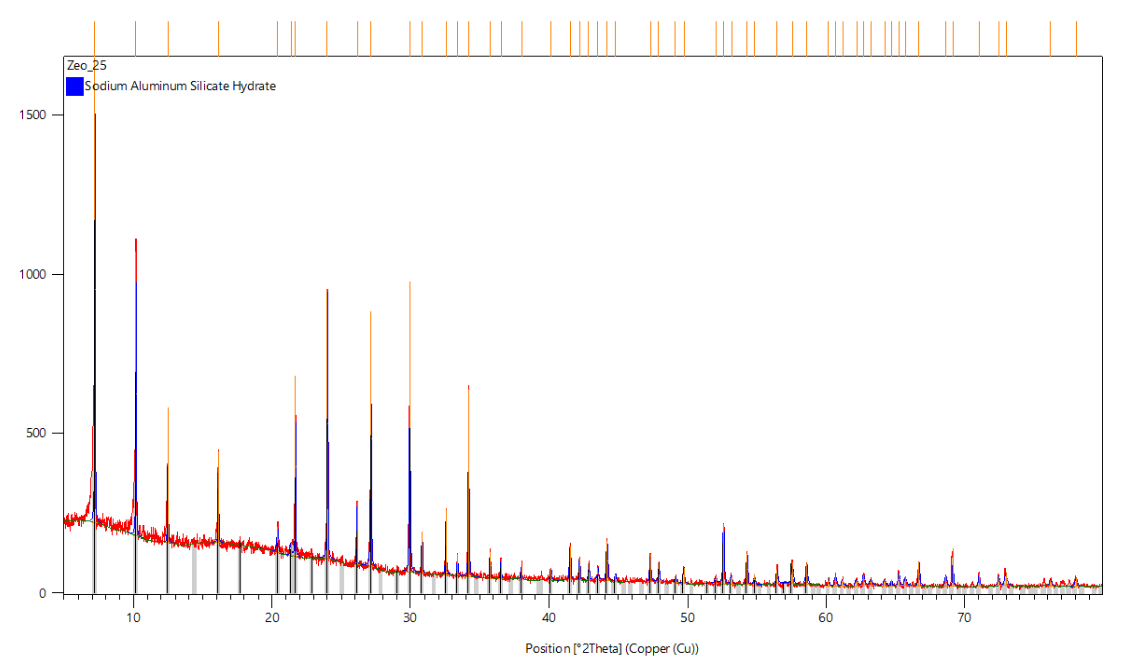
\includegraphics[scale=0.50]{Screenshot 2025-05-17 133057.png}
\end{center}
\caption{\textit{Zeigt das Pulverdiffraktogramm von hergestellten Zeolith A mit den Referenzreflexe mit dem Referenzcode 00-039-0222}}
\label{XRD}
\end{figure}
Anschließend wird mittels \mbox{HighScore-Plus} die Kristallstruktur untersucht. Dabei wurden die Einheitszelle untersucht.
Diese wurden mit den Theoretischen Werten des Referenzreflex verglichen dies wird in der Tabelle \ref{Kastenlänge} aufgezeigt.
\begin{table}[h!]
\caption{\textit{Zeigt die Theoretische und Festgestellte Einheitszelle von den hergestellten Zeolith As (Referenzcode 00-039-0222). Die Verfeinerung wurde mithilfe des Programmes HighScore Plus durchgeführt. }}
\begin{center}
\begin{tabular}{|>{\columncolor{lightgray}}>{\centering\arraybackslash}p{4cm}|>{\centering\arraybackslash}p{4cm}|>{\centering\arraybackslash}p{4cm}|}
   \hline
   \rowcolor{gray}
   &Theoretische& Festgestellte (Standardabweichung) \\
   \hline
   a[\AA]&\centering{24.6100}& 24.5847 (8)\\
   \hline
   b[\AA]&24.6100& 24.5847 (8)\\
   \hline
   c[\AA]&24.6100& 24.5847 (8)\\
   \hline
   $\alpha$[°]&90& 90\\
   \hline
   $\beta$[°]&90& 90\\
   \hline
   $\gamma$[°]&90& 90\\
   \hline
   Volumen[\AA$^3$]&14905.10 & 14859.21\\
   \hline

\end{tabular}
\label{Kastenlänge}
\end{center}
\end{table}



\subsection{\texorpdfstring{Austauschvermögen von \ce{Ca^{2+}} und \ce{Na^{+}}}{Austauschvermögen von Ca2+ und Na+}}
Zunächst wird die durchschnittliche Kristallgröße bestimmt. Dies erfolgt anhand von SEM-Aufnah-men. Dies ist in Abbildung \ref{SEm} dargestellt. Dabei handelt es sich nicht um Aufnahmen der selbst hergestellten Proben, sondern um bereitgestellte Vergleichsaufnahmen.

\begin{figure}[!h]
  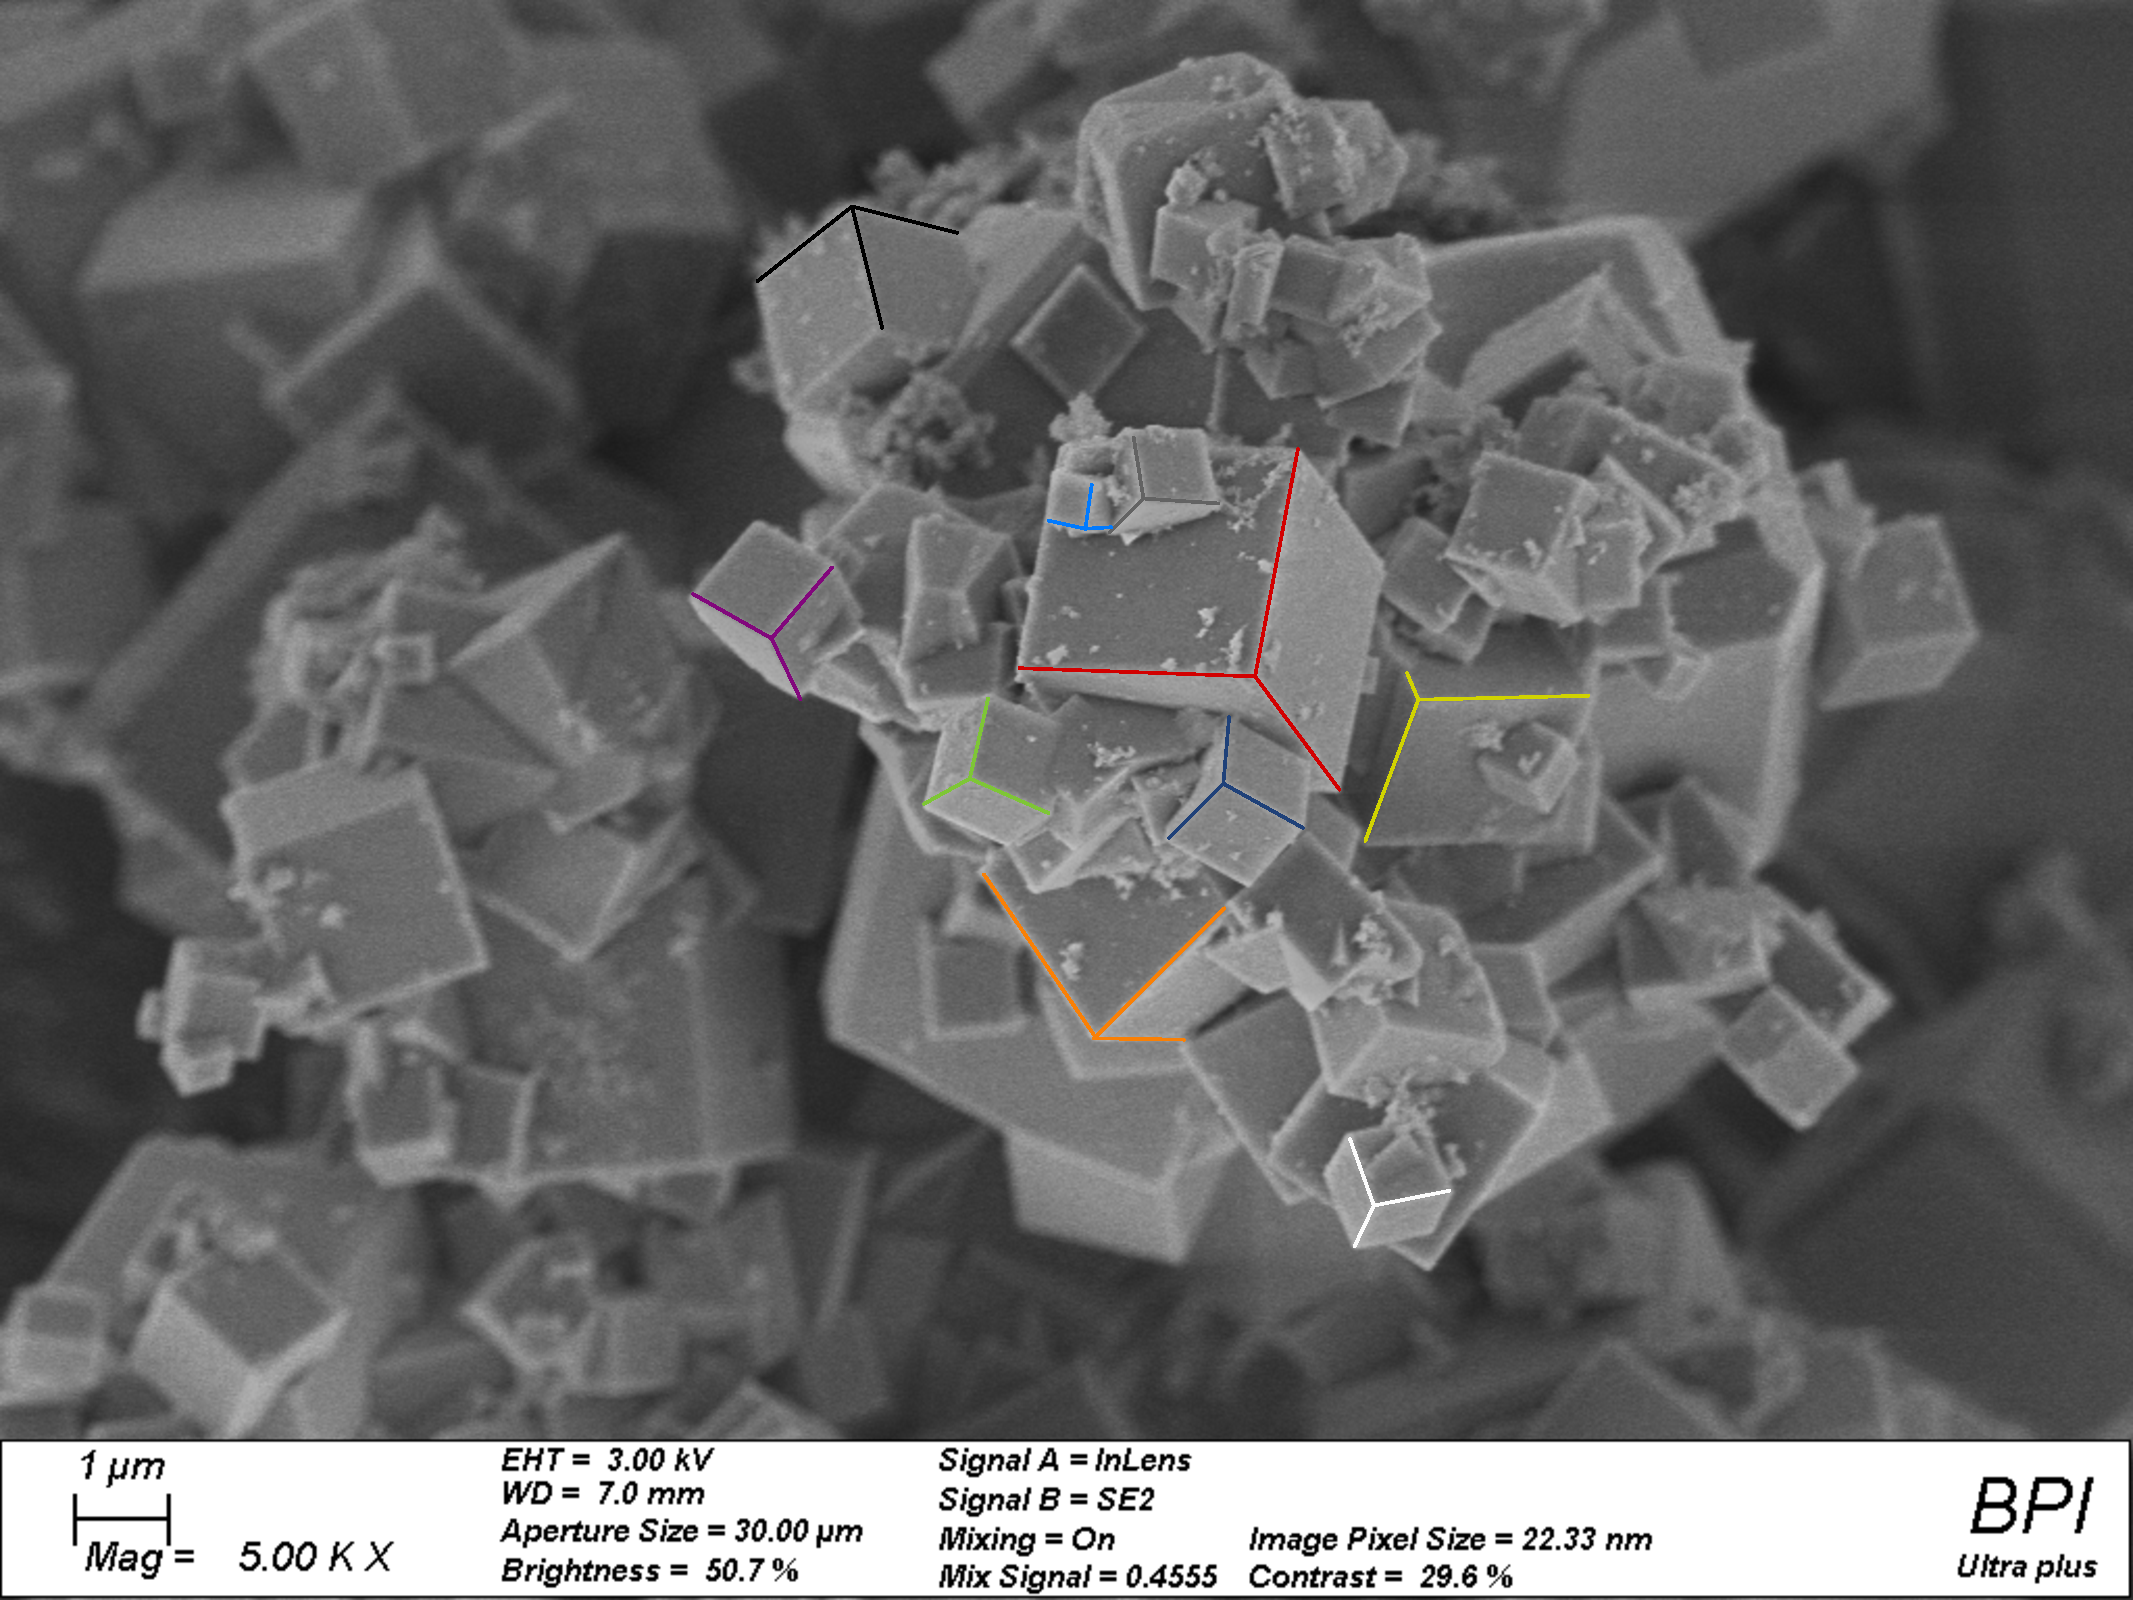
\includegraphics[width=\linewidth]{SEM_Zeo___25_.pdf}
  \caption{Zeigt die Sem-Aufnahme eines Zeolith, mit eingezeichneten Kristalle, deren Größe bestimmt werden soll.}
  \label{SEm}
\end{figure}

\noindent
Die Kristalle werden näherungsweise als Würfel angenommen. Aus der gemessenen Kantenlänge lässt sich das Kristallvolumen berechnen. Die Ergebnisse sind in Tabelle \ref{kristallgröße} dargestellt.
\newpage

\begin{table}[!h]
  \caption{zeigt die analysierten Kristalle mit den gemessenen Kantenlängen sowie den berechneten Volumina, wobei eine würfelförmige Geometrie angenommen wurde.}
  \label{kristallgröße}
\begin{tabular}{|>{\centering\arraybackslash}p{0.3\linewidth}|>{\centering\arraybackslash}p{0.3\linewidth}|>{\centering\arraybackslash}p{0.3\linewidth}|}
  \hline
  \rowcolor{gray}
  Marktierter Kristall aus der Abbildung \ref{SEm} & Kastenlänge [$\mu m$] & Volumen [$\mu m^3$]\\
  \hline
  Rot & 2.53& 16.19\\
  \hline
  Orange & 2.13 & 9.71 \\
  \hline
  Gelb & 1.80 & 5.83 \\
  \hline
  Schwarz & 1.33 & 2.37 \\
  \hline
  Lila & 1.00 & 1.00\\
 \hline
  Dunkelblau & 1.00 & 1.00\\
 \hline
  Grün & 1.00 & 1.00\\
\hline
Grau &0.80&0.51\\
\hline
Hellblau&0.40& 0.06\\
\hline
\end{tabular}

\end{table}

\noindent 
Aus der Tabelle \ref{kristallgröße} wird die Mittlere Kristallgrößes bestimmt, dieses beträgt $\overline{V} = 4.19$ $\mu $m$^3$. Daraus lässt sich 





















\newpage
\section{Zusammenfassung}




\newpage
\section{Literaturverzeichnis}
\printbibliography







\end{document}